\section{Introduction}\label{sec:Introduction}
In this note, we present the analysis for the total inclusive positively charged kaon - argon ($K^{+}$,Ar) interaction cross section for LArIAT data collected over Run-II. The note is divided into six sections. Section \ref{sec:Introduction} gives an introduction to $K$ interaction cross section measurement and its general physics context. Section \ref{sec:kaonAnalysis} provides an overview of the inclusive $K$ cross section analysis and the ``thin slice'' method. Section \ref{sec:DataSamples} lays out the data and Monte Carlo samples used in this analysis.  Section \ref{sec:BeamlineSelection} describe the LArIAT beamline and its role in the selection of the kaon-candidate events. Section \ref{sec:TPC} describes the treatment of the kaon candidates within the TPC.
Section \ref{sec:Systematics} describes the studies of the systematic uncertainties associated with the measurement. Finally, Section \ref{sec:Results} gives the results for the analysis. 

%%%%%%%%%%%%%%%%%%%%%%%%%%%%%%%%%%%%%%%%%%%%%%%%%%%%%%%%%%%%%%%%%%%%%%%%%%%%%%%%%
\subsection{Kaon interaction cross section}\label{sec:KCrossSection}
%%%%%%%%%%%%%%%%%%%%%%%%%%%%%%%%%%%%%%%%%%%%%%%%%%%%%%%%%%%%%%%%%%%%%%%%%%%%%%%%%
The interaction of a mildly relativistic charged kaon with an argon nucleus is determined largely by the strong force. The total K$^{+}$-Ar interaction cross section is defined as the one related to the single (hadronic) process driven only by the strong interaction.
In this case, ``total" indicates all strong interactions regardless of the final state. This condition purposefully includes both elastic and inelastic (reaction) channels. Indeed, the total cross section section can be then decomposed into
$$\sigma_{Tot} = \sigma_{Elastic}+ \sigma_{Reaction}.$$

For this analysis, kaons are selected from the LArIAT beamline in the momentum range between \textcolor{red}{500} MeV/c and \textcolor{red}{1000} MeV/c (see Fig \ref{fig:TOFK}).

\begin{figure}[hpbt]
\centering
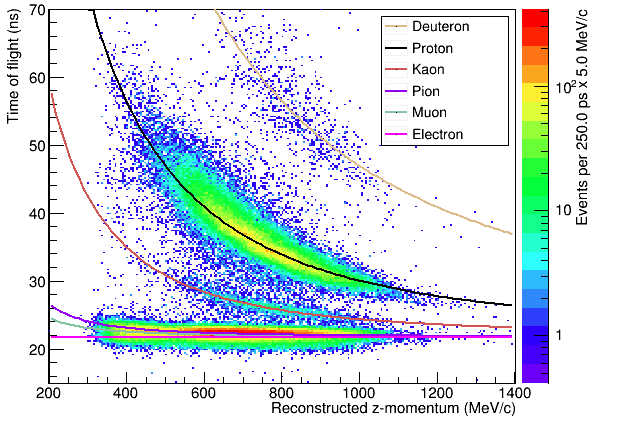
\includegraphics[width=5in]{images/Lariat/KaonTOF}
\caption{Time of flight versus momentum distributions as produced by the LArIAT TOF and Wire Chambers systems. The Kaon population lies between the proton and the muon/pion populations, allowing PID of Kaons in the beam line.  }
\label{fig:TOFK}
\end{figure}

In this energy range, the relevant K-Nucleon interactions are according to \cite{fesbach1992theoretical}:
\begin{equation}
K^{+} + N \rightarrow K^{+} + N\textit{ (elastic)}
\end{equation}
\begin{equation}K^{+} + n \rightarrow K^{0} + p\textit{ (elastic)}\end{equation}
\begin{equation}K^{+} + N \rightarrow K + N + \pi \textit{ (inelastic)}\end{equation}
\begin{equation}K^{+} + N \rightarrow K^{*} + N\textit{ (inelastic)}.\end{equation}



\subsubsection{K$^{+}$Ar Cross section in the Context of Light Mesons Interaction with Nuclei}
\label{sec:theoryStrangeMeson}
The intrinsic value of this measurement is that kaon interactions complement the measurements of $\pi$ interactions as a probe of  hadron interaction inside the nucleus in the strange sector.  
\textcolor{red}{CHIEDI REFERENZE A FLAVIO}

\subsubsection{K$^{+}$Ar Cross section in the Context of Nucleon Decay Searches}
\label{sec:theoryPDK}
Baryon number is accidentally conserved in the Standard Model. Even though no baryon number violation has been experimentally observed thus far, no underlying symmetry in line with the Noether paradigm \cite{Noether1971} explains its conservation. Almost all Grand Unified Theories predict at some level baryon number violation in the form of nucleon decay on long time-scales.  Given the impossibility to reach grand unification energy scales with collider experiments ($\sqrt{s} > 10^{15}$ GeV),  an indirect proof of GUT is needed. The experimental observation of nucleon decay may be the only viable way to explore these theories and it is therefore a subject of great interest \cite{Adams:LBNE}. %Both experiments and theory indeed suggest the energy scale for convergence of the running coupling constants of the Standard Model to be over $10^{15}$ GeV. This energy scale seems impossible to access by any foreseeable accelerator experiment, leaving baryon number violation  to be the only testable process. 

If nucleon decay was experimentally found, additional information about the GUT type may be derived from the dominant decay mode. 
Supersymmetric GUTs \cite{Dimopoulos:1981dw,Bajc20161} prefer the presence of kaons in the products of the decay, e.g. $p\rightarrow K^+\bar{\nu}$  (see fig \ref{fig:MandatoryFeynmannDiagrams}, left).
%%%%%%%%%%%%%%%% Find theory papers!!!!!! %%%%%%%%%%
Gauge mediation GUTs, in which new gauge bosons are introduced that allow for the transformation of quarks into leptons, and vice versa, prefer the mode $p\rightarrow e^+\pi^0$ (see fig \ref{fig:MandatoryFeynmannDiagrams}, right).



\begin{figure}[hbpt]
\centering
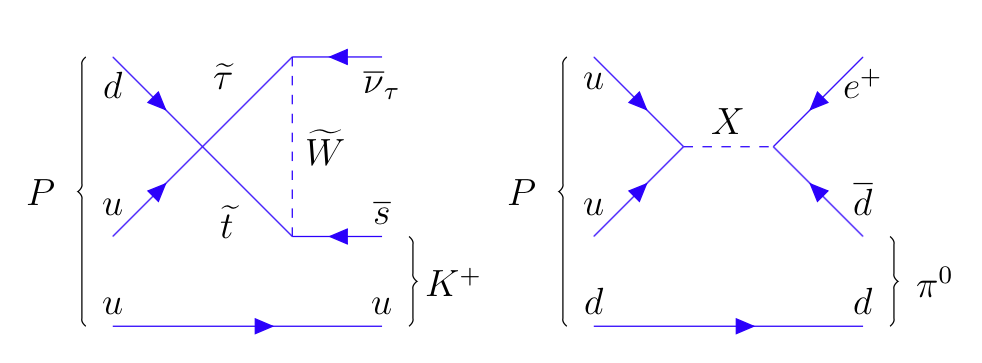
\includegraphics[width=6.5in]{images/MandatoryFeynmannDiagrams.png}
\caption{Feynman diagrams for proton decay ``golden modes": $p \rightarrow K^+ \bar{\nu}$ for supersymmetric GUTs on the left and  $p \rightarrow e^+ \pi^0$ for gauge-mediation GUTs  on the right.}
\label{fig:MandatoryFeynmannDiagrams}
\end{figure}

The key elements for a rare decay experiment are: massive active volume, long exposure, high identification efficiency and low background. 
%The limit to proton lifetime in case of absence of signal and backgrounds is set by calculating
%$$\tau/B > M\times \epsilon\times T \times 10^{32},$$ 
%where M is the detector mass in kton, $\epsilon$ the signal detection efficiency after cuts to suppress backgrounds (dependent on the considered decay mode), T is the exposure in years, B the assumed branching fraction for the considered mode and  $10^{32}$ is a factor accounting for the number of nucleons in a kton of material \cite{Bueno2007}.
Figure \ref{fig:PDKExperimentalLImit} shows the current best experimental limits on nucleon decay lifetime over branching ratio (dots). Historically, the dominant technology used in these searches has been water Cherenkov detectors: all the best experimental limits on every decay mode are indeed set by Super-Kamiokande \cite{PhysRevD.90.072005,PhysRevLett.115.121803}.  It is particularly important to notice that the kaon energy for the proton decay mode $p \rightarrow K^+ \bar{\nu}$ is under Cherenkov threshold.  Super-Kamiokande set the limit on the lifetime for the $p \rightarrow K^+ \bar{\nu}$ mode by  relying exclusively on photons from nuclear de-excitation. For this reason, an attractive alternative approach to identifying nucleon decay is the use of a Liquid Argon Time Projection Chamber (LArTPC). 

LArTPCs can complement nucleon decay searches in modes where water Cherenkov detectors are less sensitive, especially $p\rightarrow K^+\bar{\nu}$.
%The stars in Figure \ref{fig:PDKExperimentalLImit} show the projected sensitivities for new generation of nucleon decay experiments: DUNE (LArTPC) and Hyper-K (water Cherenkov).
According to \cite{Acciarri:Dune}, DUNE will have an active volume large enough, have sufficient shielding from the surface, and will run for lengths of time sufficient to compete with Hyper-K, opening up the opportunity for the discovery of nucleon decay. 

\begin{figure}[hbpt]
\centering
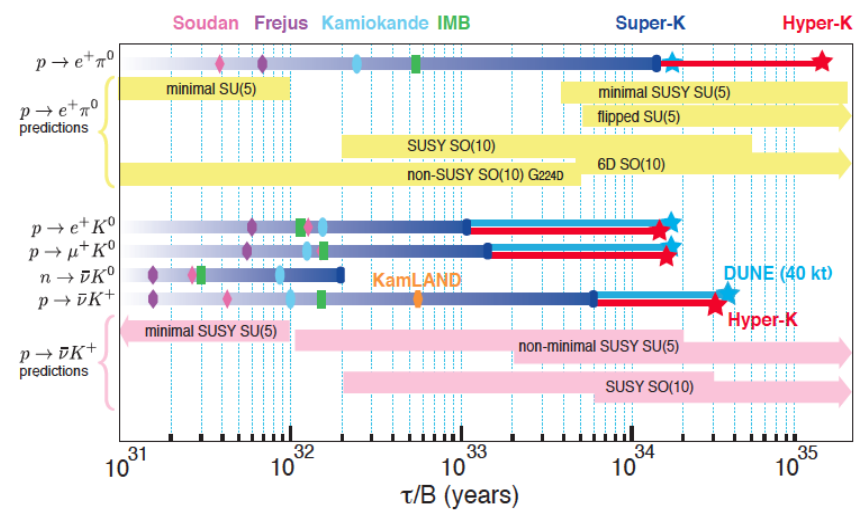
\includegraphics[width=6.5in]{images/PDKExperimentalLImit.png}
\caption{Proton decay lifetime limits from passed and future experiments.}
\label{fig:PDKExperimentalLImit}
\end{figure}

Of course, LArIAT tiny active volume makes it impossible for the experiment to place competitive limits on nucleon decay.  
However,  LArIAT provides excellent data to characterize kaons in LAr for the ``LAr golden mode" $p \rightarrow K^+ \bar{\nu}$. The result of these studies will affect future proton decay searches in LArTPCs. Previous work has been done to assess the potential identification efficiency for different decay modes in a LArTPC \cite{Bueno2007}, but, as the time of this  writing, no study of kaon selection efficiency in LArTPCs has been performed on data. 
The K$^+$-Ar interaction cross section has never been measured before and can affect the possibility of detecting and measuring kaons when produced in a proton decay event. 
Kaon interactions with argon can distort the kaon energy spectrum as well as change the topology of single kaon events. In a LArTPC, non-interacting kaons appear as straight tracks with a high ionization depositions at the end (Bragg peak). The topology of interacting kaons can be quite different. In case of elastic scattering, a distinct kink will be present in the track. In case of inelastic scattering the Bragg peak will not be present and additional tracks (pions) will populate the event.
Performing the total K$^+$-Ar cross section measurement on data serves the double purpose of identifying the rate of ``unusual" topologies (kinks and additional tracks) and of developing tools for kaon tracking in LAr.


\subsection{Previous Measurements: Lighter and Heavier Nuclei}
In general, data on kaon cross sections are  extremely scarce. The measurement of kaon interaction cross section would bring the additional benefit of reducing the uncertainties associated  with hadron interaction models adopted in MC simulations for argon targets.

The data on nuclear effects for specific hadronic final states are extremely scarce, resulting in big uncertainties in modeling final state interactions \cite{Drakoulakos:2004gn}. Figure \ref{fig:Friedmann} shows a 1997 measurement on several elements as performed by  Friedmann et al.  \cite{Friedman:1997eq}. As a reference, this paper measures a $\sigma_{Tot}$ for Si of  366.5  $\pm$  4.8 mb and a $\sigma_{Tot}$ for Ca of 494.6  $\pm$ 7.7 mb at 488 MeV/c.  The cross section for argon is expected to lie in between these two measurements. 
Additional data on the kaon cross section are provided by Bugg et al. \cite{PhysRev.168.1466}. Bugg performs a measurement of the total 
K$^+$ and K$^-$ cross sections on protons and deuterons over the range of 0.6-2.65 GeV/c, as well as a measurement of the total K$^+$ and K$^-$  cross sections on carbon for a number of momenta; the results of this paper on carbon are reported in Figure \ref{fig:Bugg}.




\begin{figure}
\captionsetup{justification=raggedright}  
\begin{minipage}[b]{.5\textwidth}  
  \centering  
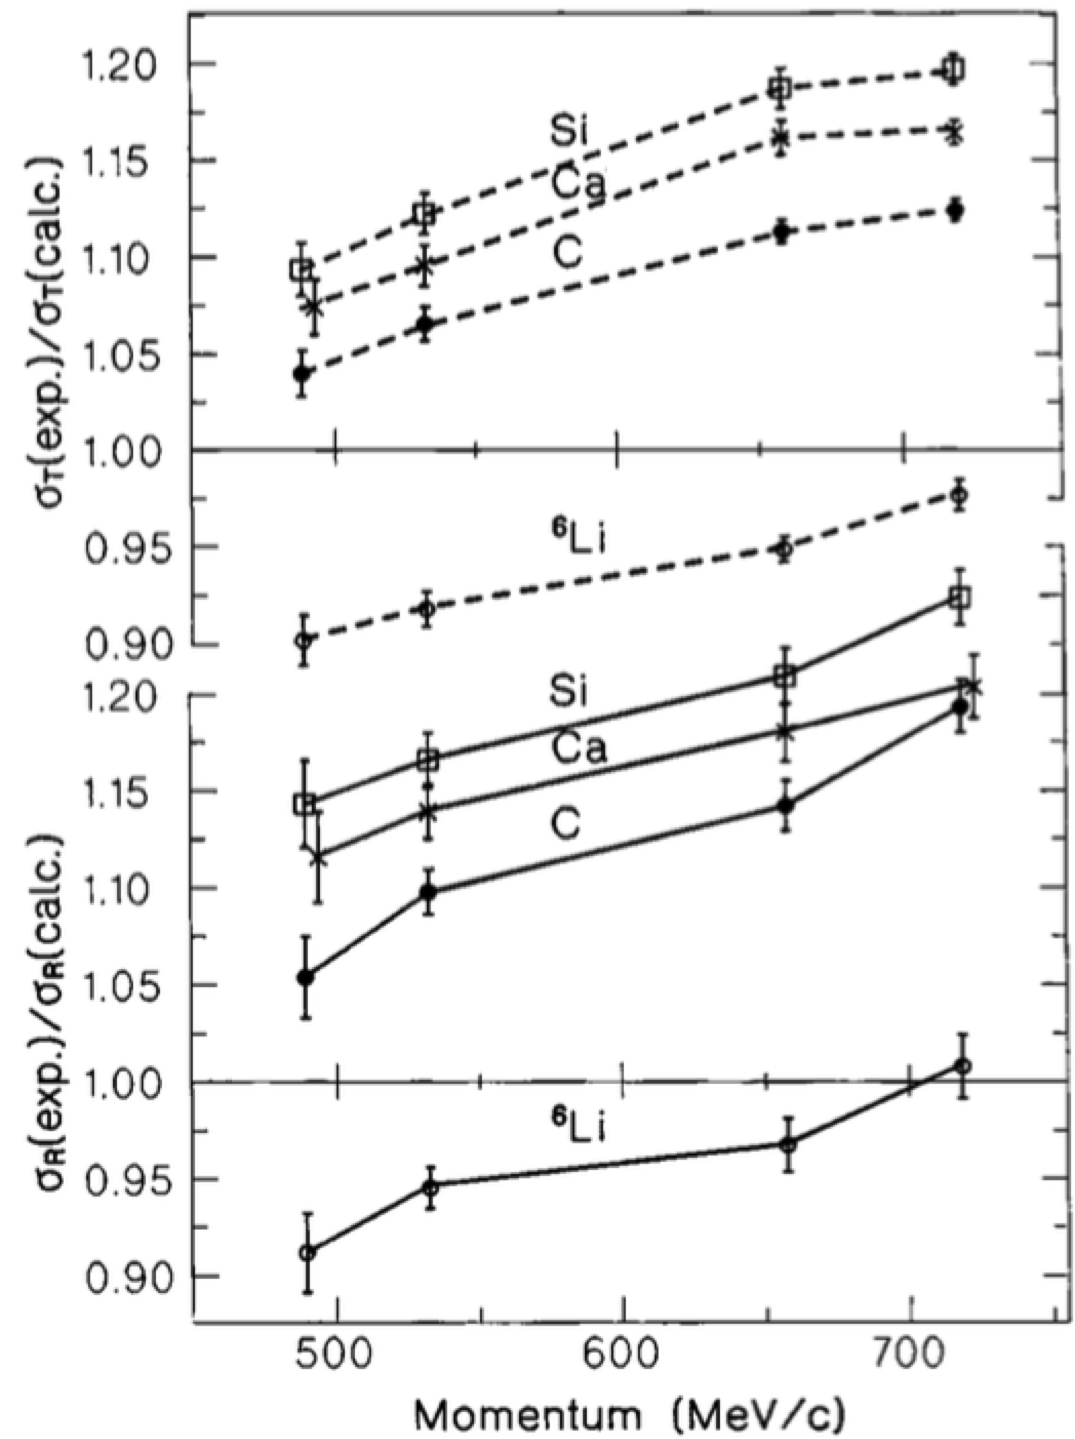
\includegraphics[width=3in]{images/Lariat/Friedmann.png}
\end{minipage}%  
\begin{minipage}[b]{0.5\textwidth}  
  \centering  
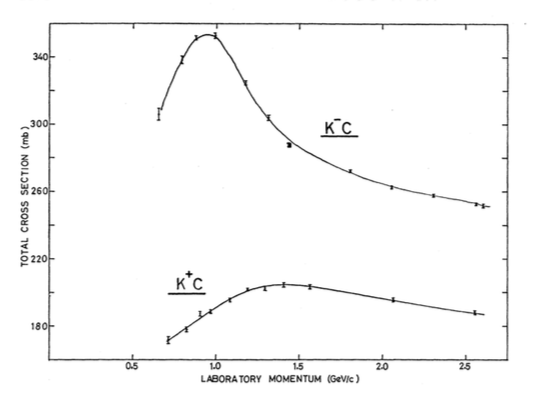
\includegraphics[width=3in]{images/Lariat/Bugg.png}
\end{minipage}
\par
\begin{minipage}[t]{.53\textwidth}
\caption{Ratios between experimental and calculated cross sections as from \cite{Friedman:1997eq}. Top: Total cross sections. Bottom: reaction cross sections.}
\label{fig:Friedmann}
\end{minipage}%
\begin{minipage}[t]{.5\textwidth}  
\caption{Total K$^+$  and K$^-$ cross sections on carbon as from \cite{PhysRev.168.1466}.}
\label{fig:Bugg}
\end{minipage}  
\end{figure}



%%%%%%%%%%%%%%%%%%%%%%%%%%%%%%%%%%%%%%%%%%%%%%%%%%%%%%%
%% PRETTY EVENT DISPLAY WITH TEXT, NOT SURE IF USEFUL
%\begin{figure}[h!]
%\centering
%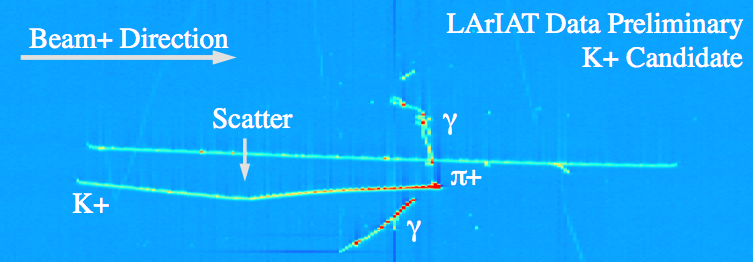
\includegraphics[width=6.5in]{images/Lariat/KLariat.png}
%\caption{LArIAT Data $K^+$ candidate. $K^+$ enters TPC, undergoes a hadronic scatter, and then decays into $\pi^+$ and $\pi^0$. The the $\pi^0$ decays into 2 photons while the $\pi^+$ stops quickly in the TPC. Collection plane view.}
%\label{Fig:KLariat}
%\end{figure}

%Fig \ref{Fig:KLariat} shows a $K^+$ candidate event in the LArIAT TPC. Following the kaon candidate track from left to right, two important elements are visible by eye: a change in the K momentum due to hadronic scatter and a Bragg peak by the end of the track due to an augment of ionization as the kaon slows down in the TPC. The track "kink" is only visible thanks to the millimetric spacial resolution of the TPC, while the Bragg shows the calorimetric power of this technology. The kaon in this event decays hadronically into $\pi^+$ and $\pi^0$. The the $\pi^0$ decays into 2 photons while the $\pi^+$ stops quickly in the TPC. The ability to distinguish the topology of this decay from the most frequent one, i.e. $K^+\rightarrow\mu^+\nu$, remarks the versatility of the LArTPC technology.
%%%%%%%%%%%%%%%%%%%%%%%%%%%%%%%%%%%%%%%%%%%%%%%%%%%%%%%




 \subsection{Kaon Interaction Cross Section for thin target in Geant4}
Since the kaon cross section in argon has never been measured before, the Geant4 Monte Carlo tunes kaon transportation in argon by extrapolation from lighter and heavier nuclei. As shown in the previous section,  kaon data on carbon are available and  can be used as a metric to evaluate the Geant4 prediction performances.  Figure \ref{fig:TrueCarbon} shows the total hadronic cross section for carbon implemented in Geant4 10.01.p3 overlaid with the Bugg and Friedman data. Unfortunately, the current version of Geant4 does not reproduce the data for carbon closely. On one hand, this evidence makes us even more wary when using the Monte Carlo in simulating the kaon-argon interactions. On the other, it further highlights the importance of kaon measurements.

The K$^{+}$Ar cross section implemented in Geant4 can still be used as a tool to validate the measurement methodology. For the considered energy range, the Geant4 inelastic model adopted to is ``BertiniCascade", while the elastic model ``hElasticLHEP".  Figure \ref{fig:TrueArgon} shows the total hadronic cross section for argon implemented in Geant4 10.01.p3 (solid lines) overlaid with the true MC cross section as obtained with the sliced TPC method (markers); the total cross section is shown in green,  the elastic cross section in blue and the inelastic cross section in red. The sliced TPC method described in sec \ref{sec:KXSStrategy}. For the methodology validation we use the true energy deposition for a pool of about 140000 kaons fired inside the LArIAT TPC active volume and a uniform slice length of 4.7 mm.  The nice agreement with the Geant4 distribution and the cross section  obtained with the sliced TPC method gives us confidence in the  validity of the methodology. 
        
     
\begin{figure}
\captionsetup{justification=raggedright}  
\begin{minipage}[b]{.53\textwidth}  
  \centering  
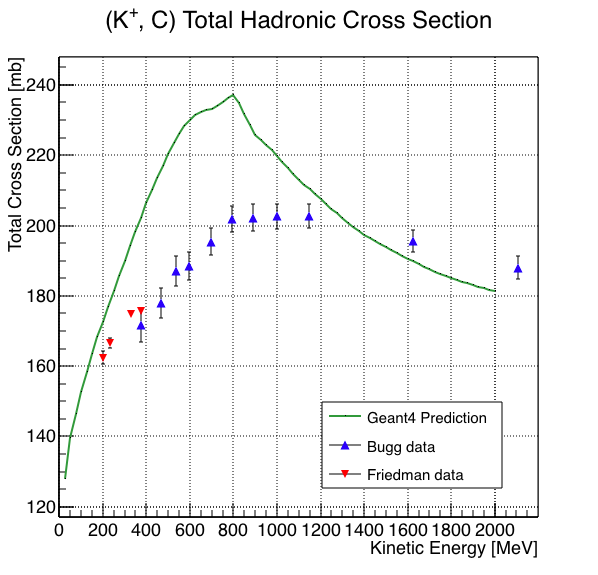
\includegraphics[width=3in]{images/Lariat/CarbonG4.png}
\end{minipage}%  
\begin{minipage}[b]{0.53\textwidth}  
  \centering  
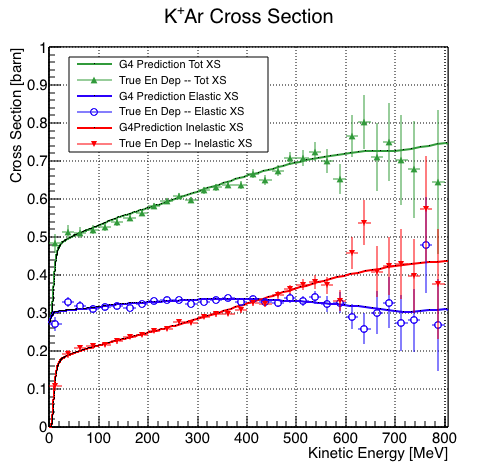
\includegraphics[width=3in]{images/Lariat/KaonTrueXS.png}
\end{minipage}
\par
\begin{minipage}[t]{.53\textwidth}
\caption{total hadronic cross section for carbon implemented in Geant4  10.01.p3  with overlaid with the Bugg and Frideman data.}
\label{fig:TrueCarbon}
\end{minipage}%
\begin{minipage}[t]{.5\textwidth}  
\caption{Hadronic cross sections for argon implemented in Geant4 10.01.p3 (solid lines) overlaid the true MC cross section as obtained with the sliced TPC method (markers). The total cross section is shown in green,  the elastic cross section in blue and the inelastic cross section in red.}
\label{fig:TrueArgon}
\end{minipage}  
\end{figure}




